\section{Organisatorisches}

Prof. Gorbunoff

Literaturempfehlung: Werkstoffe der Elektrotechnik Ivers-Tiffeé von Münch Teubner

Zur Prüfung ist alles ausschließlich handschriftliche zugelassen.

\section{Werkstoffeigenschaften}

\begin{tabular}{c c c c}
	Eigenschaft & Stimulus & typische Reaktion & Kenngröße \\
	\hline
	mechanische & mechanische Kraft & Verformung, Bruch & $E$, $\sigma$ \\
	thermische & Energiezufuhr & Temperaturanstieg & $C_v$, $\lambda$ \\
	elektrische & E-Feld & Strom, Polarisation & $p$, $\epsilon$ \\
	optische & Licht & Farbe, Brechung & $R$, $T$, $n$ \\
	magnetische & H-Feld & magnetische Anziehung & $\mu$, $H_c$\\
\end{tabular}

Werkstoffe mit mechanischen Eigenschaften sind Konstruktionswerkstoffe. Die anderen sind Funktionswerkstoffe.

\subsection{Aufbau der Atome und Periodensystem der Elemente}

\subsubsection{Bohr'sches Atommodell und Wasserstoffatom}

\begin{minipage}{.3\textwidth}
	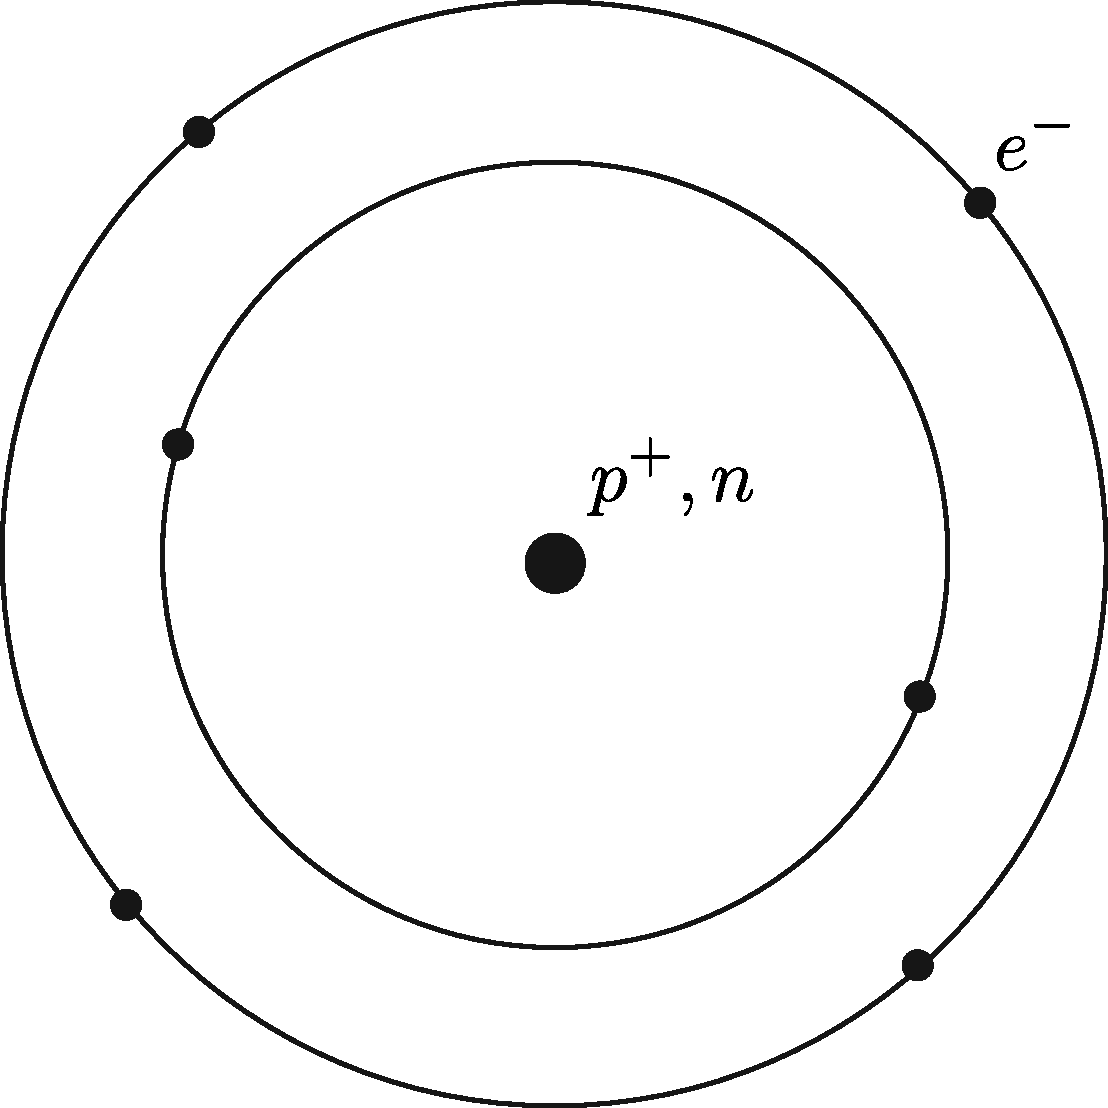
\includegraphics[width=\textwidth]{img/1_1}
\end{minipage}\hfill
\begin{minipage}{.65\textwidth}
	\begin{itemize}
		\item Kern: ca. $10^{-5}...10^{-4} \angstrom$ ($1\angstrom = 10^{-10}m$)
		\begin{itemize}
			\item Neutronen ($n$): $q_n = 0$
			\item Protonen ($p^+$): $q_p = e = 1{,}60 \cdot 10^{-19}C$
		\end{itemize}
		\item Elektronenhülle: R ca. $0{,}5...2{,}5\angstrom$
		\begin{itemize}
			\item Elektronen ($e^-$): $q_e = -e = -1{,}60 \cdot 10^{-19}C$ \\ 
			$m_e << m_n$ \Ra Die ganze Masse des Atoms ist nahezu im Kern konzentriert.
		\end{itemize}
		\item Orbital: Aufenthaltsraum des Elektrons im Raum
	\end{itemize}
\end{minipage}

\underbar{Energieniveaus von Elektronen in Atomen}

Wenn Elektronen von einem Orbital zu einem anderen springen, entstehen Protonen oder werden absorbiert. \ra Diese Übergänge sind also reversibel.

Atome haben diskrete Energieniveaus (Orbitale). Atome müssen nicht neutral sein.

Diskrete Energieniveaus: Bindungsenergien von Elektronen im Atom

Valenzelektronen (ganz außen) haben die geringsten Bindungsenergien.

\subsubsection{Quantenmechanik und die Elektronenhülle}

<Buch 1.3>

Alle Elektronen mit der selben Hauptquantenzahl ($n$) bilden eine Elektronenschale (K-Schale ist die innerste).

Die Bahndrehimpulsquantenzahl ($l$) bestimmt die Form.
\begin{itemize}
	\item liegt zwischen 0 und $n-1$
	\item alle Elektronen mit der selben Nebenquantenzahl (Bahndrehimpuls-QZ) bilden eine Unterschale.
\end{itemize}

Orientierungsquantenzahl ($m_l$)
\begin{itemize}
	\item bestimmt räumliche Orientierung
	\item betrifft nur nicht-kugelförmige Orbitale
	\item ganzzahlig, positiv oder negativ, zwischen 0 und $\pm l$
\end{itemize}

\underbar{Besetzung der Elektronenzustände}
\begin{itemize}
	\item Prinzip der Energieminimierung\\
		Ein Elektron besetzt bei mehreren Möglichkeiten das Orbital mit der niedrigsten Energie, d.h. meist das innerste
	\item Pauli-Ausschließungsprinzip \\
		In einem Atom dürfen keine zwei \underbar{identischen} Elektronen einen und denselben Quantenzustand besitzen. Elektronen unterscheiden sich in erster Linie im Spin.
\end{itemize}

Eigendrehimpulsquantenzahl ($m_s$) ``\textit{Spin}''
\begin{itemize}
	\item positiv oder negativ $\frac{1}{2}$ (``spin up'', ``spin down'')
\end{itemize}
\Ra mit zwei Elektronen mit unterschiedlichem Spin ist die K-Schale voll besetzt, da sie nur eine Unterschale hat.

<Buch 1.4>

<Buch 1.9>

Nach 3p kommt 4s, da 4s ein tieferes Niveau hat als 3d.

\subsubsection{Das Periodensystem der Elemente}

Das Periodensystem spiegelt die Besetzungsreihenfolge der Elektronen.
